% General-purpose named IEEE-style conference manuscript.
% Generated from the maintained conference working source.
\documentclass[conference]{IEEEtran}
    \IEEEoverridecommandlockouts

    \usepackage{cite}
    \usepackage{amsmath,amssymb,amsfonts}
    \usepackage{algorithm}
    \usepackage{algpseudocode}
    \usepackage{graphicx}
    \usepackage{booktabs}
    \usepackage{array}
    \usepackage{multirow}
    \usepackage{xcolor}
    \usepackage{url}
    \usepackage[hidelinks]{hyperref}
    \usepackage{microtype}

    % Generated numerical artifacts. These files are produced by the scripts in
    % paper/ and should be regenerated before submission.
    % Auto-generated by paper/make_figures.py -- do not edit by hand.
\newcommand{\totalBill}{2189.48}
\newcommand{\totalSavings}{590.40}
\newcommand{\savingsPctBill}{27.0}
\newcommand{\savingsPctBillExact}{26.97}
\newcommand{\savingsPctFlagged}{54.9}
\newcommand{\flaggedCost}{1074.83}
\newcommand{\afterCost}{484.43}
\newcommand{\numRecs}{19}
\newcommand{\numAiRecs}{10}
\newcommand{\numEctwo}{8}
\newcommand{\numResources}{42}
\newcommand{\numServicesBilled}{6}
\newcommand{\nDays}{365}
\newcommand{\dataStart}{2024-07-01}
\newcommand{\dataEnd}{2025-06-30}
\newcommand{\meanDaily}{74.64}
\newcommand{\stdDaily}{22.87}
\newcommand{\minDaily}{36.10}
\newcommand{\maxDaily}{232.52}
\newcommand{\annualTotal}{27,243.31}
\newcommand{\surgeThresh}{120.38}
\newcommand{\numSurges}{5}
\newcommand{\maxZ}{6.9}
\newcommand{\savRightsize}{362.81}
\newcommand{\cntRightsize}{2}
\newcommand{\savPricing}{208.42}
\newcommand{\cntPricing}{6}
\newcommand{\savDelete}{10.00}
\newcommand{\cntDelete}{3}
\newcommand{\savNat}{5.67}
\newcommand{\cntNat}{2}
\newcommand{\savEbs}{2.60}
\newcommand{\cntEbs}{4}
\newcommand{\savSthree}{0.79}
\newcommand{\cntSthree}{1}
\newcommand{\savLambda}{0.11}
\newcommand{\cntLambda}{1}
\newcommand{\savHigh}{370.52}
\newcommand{\cntHigh}{8}
\newcommand{\savMed}{214.21}
\newcommand{\cntMed}{9}
\newcommand{\savLow}{5.67}
\newcommand{\cntLow}{2}
\newcommand{\mapeSnaive}{12.3}
\newcommand{\mapeEts}{11.2}
\newcommand{\mapeProphet}{20.9}
\newcommand{\mapeNaive}{27.3}
\newcommand{\bestModel}{ETS}
\newcommand{\bestMape}{11.2}
\newcommand{\holdoutModel}{ETS}
\newcommand{\holdoutMape}{12.0}
\newcommand{\holdoutCov}{97}
\newcommand{\cvInitial}{120}
\newcommand{\cvStep}{30}

    % Auto-generated by paper/external_validation.py -- do not edit by hand.
\newcommand{\extSnapshot}{2026-06-30}
\newcommand{\extCatalogSize}{28}
\newcommand{\extFsVms}{1250}
\newcommand{\extFsBaseline}{128,588}
\newcommand{\extFsOptimized}{85,414}
\newcommand{\extFsSavingsPct}{33.6}
\newcommand{\extFsSavingsPctRi}{58.3}
\newcommand{\extFsDownsized}{765}
\newcommand{\extFsUpsized}{181}
\newcommand{\extFsClamped}{0}
\newcommand{\extRndVms}{500}
\newcommand{\extRndBaseline}{44,294}
\newcommand{\extRndOptimized}{29,614}
\newcommand{\extRndSavingsPct}{33.1}
\newcommand{\extRndSavingsPctRi}{58.0}
\newcommand{\extRndDownsized}{301}
\newcommand{\extRndUpsized}{57}
\newcommand{\extRndClamped}{0}
\newcommand{\extMatVms}{547}
\newcommand{\extMatBaseline}{44,184}
\newcommand{\extMatOptimized}{11,398}
\newcommand{\extMatSavingsPct}{74.2}
\newcommand{\extMatSavingsPctRi}{83.8}
\newcommand{\extMatDownsized}{509}
\newcommand{\extMatUpsized}{4}
\newcommand{\extMatClamped}{0}
\newcommand{\extGammaReal}{0.63}
\newcommand{\extTotalVms}{2,297}
\newcommand{\extRndHours}{2142}
\newcommand{\extRndMeanGhz}{402.4}
\newcommand{\extRndSurges}{149}
\newcommand{\extMapeNaive}{82.3}
\newcommand{\extMapeSdNaive}{66.6}
\newcommand{\extMaseNaive}{0.91}
\newcommand{\extCovNaive}{95}
\newcommand{\extMapeSnaive}{65.0}
\newcommand{\extMapeSdSnaive}{40.3}
\newcommand{\extMaseSnaive}{1.35}
\newcommand{\extCovSnaive}{74}
\newcommand{\extMapeEts}{77.0}
\newcommand{\extMapeSdEts}{57.2}
\newcommand{\extMaseEts}{0.93}
\newcommand{\extCovEts}{54}
\newcommand{\extMapeProphet}{60.8}
\newcommand{\extMapeSdProphet}{21.6}
\newcommand{\extMaseProphet}{1.01}
\newcommand{\extCovProphet}{62}
\newcommand{\extBestModel}{Prophet}
\newcommand{\extBestMape}{60.8}
\newcommand{\extNFolds}{9}
\newcommand{\extDmStat}{-1.20}
\newcommand{\extDmP}{0.232}
\newcommand{\extWilcoxonP}{0.570}
\newcommand{\extDmPProphetSnaive}{0.235}
\newcommand{\extDmPProphetNaive}{0.604}
\newcommand{\extAnyBestMape}{48.2}
\newcommand{\extDailyMapeNaive}{53.4}
\newcommand{\extDailyMapeSdNaive}{14.2}
\newcommand{\extDailyMaseNaive}{1.32}
\newcommand{\extDailyMapeSnaive}{54.2}
\newcommand{\extDailyMapeSdSnaive}{22.6}
\newcommand{\extDailyMaseSnaive}{1.26}
\newcommand{\extDailyMapeEts}{52.1}
\newcommand{\extDailyMapeSdEts}{29.9}
\newcommand{\extDailyMaseEts}{1.10}
\newcommand{\extDailyMapeProphet}{59.8}
\newcommand{\extDailyMapeSdProphet}{36.9}
\newcommand{\extDailyMaseProphet}{1.26}
\newcommand{\extDailyBestModel}{ETS}
\newcommand{\extDailyBestMape}{52.1}
\newcommand{\extDailyNFolds}{7}
% Additional Study II reproducibility macros from paper/study2_reproducibility.py.
\newcommand{\extFsSavingsCiLow}{24.5}
\newcommand{\extFsSavingsCiHigh}{41.8}
\newcommand{\extFsSavingsPctRiCiLow}{52.5}
\newcommand{\extFsSavingsPctRiCiHigh}{63.5}
\newcommand{\extRndSavingsCiLow}{19.3}
\newcommand{\extRndSavingsCiHigh}{46.3}
\newcommand{\extRndSavingsPctRiCiLow}{49.3}
\newcommand{\extRndSavingsPctRiCiHigh}{66.3}
\newcommand{\extMatSavingsCiLow}{71.4}
\newcommand{\extMatSavingsCiHigh}{76.8}
\newcommand{\extMatSavingsPctRiCiLow}{82.1}
\newcommand{\extMatSavingsPctRiCiHigh}{85.4}
\newcommand{\extOverallSavingsPct}{41.8}
\newcommand{\extOverallSavingsCiLow}{35.9}
\newcommand{\extOverallSavingsCiHigh}{47.5}
\newcommand{\extOverallSavingsPctRi}{63.4}
\newcommand{\extOverallSavingsPctRiCiLow}{59.7}
\newcommand{\extOverallSavingsPctRiCiHigh}{67.0}

    % Auto-generated by paper/azure_validation.py -- do not edit by hand.
\newcommand{\azVms}{237,272}
\newcommand{\azTotalRows}{2,695,548}
\newcommand{\azDroppedBucket}{10,923}
\newcommand{\azDroppedShort}{2,447,247}
\newcommand{\azBaseline}{16,670,839}
\newcommand{\azOptimized}{17,307,607}
\newcommand{\azSavingsPct}{-3.8}
\newcommand{\azSavingsPctRi}{34.8}
\newcommand{\azDownsized}{21,772}
\newcommand{\azUpsized}{26,227}

    % Auto-generated by paper/policy_sim.py -- do not edit by hand.
\newcommand{\polGammaStar}{0.63}
\newcommand{\polTrainPeriods}{219}
\newcommand{\polTestPeriods}{146}
% Deprecated *Days aliases retained for finalized conference/main consumers; values count periods (sampling period: day). Use *Periods in new prose.
\newcommand{\polTrainDays}{219}
\newcommand{\polTestDays}{146}
\newcommand{\polPctHeur}{101.8}
\newcommand{\polPctNv}{73.6}
\newcommand{\polPctSaa}{73.6}
\newcommand{\polPctLookSeven}{74.1}
\newcommand{\polPctLookThirty}{73.3}
\newcommand{\polPctLookSixty}{73.4}
\newcommand{\polPctDual}{72.8}
\newcommand{\polPctDualc}{74.6}
\newcommand{\polPctLb}{63.0}
\newcommand{\polPoC}{28.2}
\newcommand{\polImpliedQ}{99}
\newcommand{\polSurgeTrain}{3}
\newcommand{\polSurgeTest}{2}
\newcommand{\polNvSave}{26.4}
\newcommand{\polDualGain}{0.8}
\newcommand{\polDualcGain}{-1.0}
\newcommand{\polDualGapCapture}{7}
\newcommand{\polDualcGapCapture}{-10}
\newcommand{\polHeurBreakeven}{0.62}
\newcommand{\polDualGainThreshMin}{-0.6}
\newcommand{\polDualGainThreshMax}{0.8}
\newcommand{\polDualcGainThreshMin}{-3.0}
\newcommand{\polDualcGainThreshMax}{-1.0}
\newcommand{\polDualcGainHoldOne}{-1.0}
\newcommand{\polNvSaveMin}{26.1}
\newcommand{\polNvSaveMax}{26.4}
\newcommand{\polPoCMin}{22.6}
\newcommand{\polPoCMax}{28.2}
% Empirical commitment-proxy Q values; units are arm-specific.
\newcommand{\polQheur}{125.3}
\newcommand{\polQnv}{68.8}
\newcommand{\polQlookSeven}{82.0}
\newcommand{\polQlookThirty}{73.1}
\newcommand{\polQlookSixty}{72.7}
\newcommand{\polLookSevenPeriods}{7}
\newcommand{\polLookThirtyPeriods}{30}
\newcommand{\polLookSixtyPeriods}{60}
\newcommand{\polQdualbase}{68.5}
\newcommand{\polQdualsurge}{195.7}
% Deprecated K-named aliases for finalized conference/main consumers.
\newcommand{\polKheur}{\polQheur}
\newcommand{\polKnv}{\polQnv}
\newcommand{\polKlookSeven}{\polQlookSeven}
\newcommand{\polKlookThirty}{\polQlookThirty}
\newcommand{\polKlookSixty}{\polQlookSixty}
\newcommand{\polKdualbase}{\polQdualbase}
\newcommand{\polKdualsurge}{\polQdualsurge}
\newcommand{\polSaaNvGapPct}{0.57}
\newcommand{\polOdMonthly}{2,388.62}
\newcommand{\polHeurMonthly}{2,432.01}
\newcommand{\polNvMonthly}{1,757.46}
\newcommand{\polPoCMonthly}{674.55}

    % Auto-generated by paper/policy_sim.py -- do not edit by hand.
\newcommand{\extPolGammaStar}{0.63}
\newcommand{\extPolTrainPeriods}{1285}
\newcommand{\extPolTestPeriods}{857}
% Deprecated *Days aliases retained for finalized conference/main consumers; values count periods (sampling period: hour). Use *Periods in new prose.
\newcommand{\extPolTrainDays}{1285}
\newcommand{\extPolTestDays}{857}
\newcommand{\extPolPctHeur}{153.5}
\newcommand{\extPolPctNv}{86.2}
\newcommand{\extPolPctSaa}{86.2}
\newcommand{\extPolPctLookSeven}{91.2}
\newcommand{\extPolPctLookThirty}{84.9}
\newcommand{\extPolPctLookSixty}{86.2}
\newcommand{\extPolPctDual}{77.7}
\newcommand{\extPolPctDualc}{78.1}
\newcommand{\extPolPctLb}{63.0}
\newcommand{\extPolPoC}{67.4}
\newcommand{\extPolImpliedQ}{100}
\newcommand{\extPolSurgeTrain}{54}
\newcommand{\extPolSurgeTest}{124}
\newcommand{\extPolNvSave}{13.8}
\newcommand{\extPolDualGain}{8.5}
\newcommand{\extPolDualcGain}{8.1}
\newcommand{\extPolDualGapCapture}{37}
\newcommand{\extPolDualcGapCapture}{35}
\newcommand{\extPolDualGainThreshMin}{2.8}
\newcommand{\extPolDualGainThreshMax}{8.5}
\newcommand{\extPolDualcGainThreshMin}{2.7}
\newcommand{\extPolDualcGainThreshMax}{8.1}
\newcommand{\extPolDualcGainHoldOne}{8.1}
\newcommand{\extPolNvSaveMin}{12.5}
\newcommand{\extPolNvSaveMax}{16.0}
\newcommand{\extPolPoCMin}{45.8}
\newcommand{\extPolPoCMax}{116.4}
% Empirical commitment-proxy Q values; units are arm-specific.
\newcommand{\extPolQheur}{1096248.9}
\newcommand{\extPolQnv}{203631.6}
\newcommand{\extPolQlookSeven}{511981.0}
\newcommand{\extPolQlookThirty}{268870.3}
\newcommand{\extPolQlookSixty}{203631.6}
\newcommand{\extPolLookSevenPeriods}{168}
\newcommand{\extPolLookThirtyPeriods}{720}
\newcommand{\extPolLookSixtyPeriods}{1285}
\newcommand{\extPolQdualbase}{197302.0}
\newcommand{\extPolQdualsurge}{936657.4}
% Deprecated K-named aliases for finalized conference/main consumers.
\newcommand{\extPolKheur}{\extPolQheur}
\newcommand{\extPolKnv}{\extPolQnv}
\newcommand{\extPolKlookSeven}{\extPolQlookSeven}
\newcommand{\extPolKlookThirty}{\extPolQlookThirty}
\newcommand{\extPolKlookSixty}{\extPolQlookSixty}
\newcommand{\extPolKdualbase}{\extPolQdualbase}
\newcommand{\extPolKdualsurge}{\extPolQdualsurge}
\newcommand{\extPolSaaNvGapPct}{0.12}

    % Auto-generated by paper/evidence_experiments.py -- do not edit by hand.
\newcommand{\evidComputeCurrent}{1241.58}
\newcommand{\evidPfiveCost}{1005.65}
\newcommand{\evidPfiveSavingsPct}{19.0}
\newcommand{\evidPfiveSavingsPctExact}{19.003}
\newcommand{\evidEcTwoCurrent}{843.73}
\newcommand{\evidEcTwoOptimized}{970.61}
\newcommand{\evidEcTwoDelta}{126.87}
\newcommand{\evidEcTwoDeltaPct}{15.0}
\newcommand{\evidRdsCurrent}{397.85}
\newcommand{\evidRdsOptimized}{35.04}
\newcommand{\evidRdsDelta}{-362.81}
\newcommand{\evidRdsDeltaPct}{-91.2}
\newcommand{\evidRdsSavings}{362.81}
\newcommand{\evidRdsSavingsPct}{91.2}
\newcommand{\evidAggregateDelta}{-235.93}
\newcommand{\evidAggregateDeltaPct}{-19.0}
\newcommand{\evidAggregateSavings}{235.93}
% Deprecated \evidCommercial* packaging aliases retained for finalized conference/main consumers.
\newcommand{\evidCommercialLookback}{7/30/60}
\newcommand{\evidCommercialLookbacks}{7/30/60}
\newcommand{\evidCommercialRecs}{6}
\newcommand{\evidCommercialCurrent}{563.42}
\newcommand{\evidCommercialSavings}{209.15}
\newcommand{\evidCommercialSavingsPct}{37.1}
\newcommand{\evidRiReplayLookback}{7/30/60}
\newcommand{\evidRiReplayLookbacks}{7/30/60}
\newcommand{\evidRiReplayRecs}{6}
\newcommand{\evidRiReplayCurrent}{563.42}
\newcommand{\evidRiReplaySavings}{209.15}
\newcommand{\evidRiReplaySavingsPct}{37.1}
\newcommand{\evidRuleRecs}{15}
\newcommand{\evidRuleSavings}{507.83}


    \newcommand{\E}{\mathbb{E}}
    \newcommand{\pos}[1]{\left(#1\right)^+}
    \graphicspath{{../figures/}}

    \hypersetup{
      pdftitle={The Price of Conservatism in Cloud Optimization: Empirical Evidence from Right-Sizing and Reservation Heuristics},
      pdfauthor={Ibrahim Mohamed; Mariam Emad; Hazem Ibrahim; Ahmed Sameh; Mahmoud Ahmed; John Ehab},
      pdfsubject={Cloud cost optimization, right-sizing, and reservation heuristics},
      pdfkeywords={cloud cost optimization, right-sizing, capacity reservation, resource management, cloud pricing, workload traces, FinOps, empirical evaluation}
    }

    \begin{document}

    \title{The Price of Conservatism in Cloud Optimization: Empirical Evidence from Right-Sizing and Reservation Heuristics}

    \author{
    \IEEEauthorblockN{\small Ibrahim Mohamed, Mariam Emad, Hazem Ibrahim, Ahmed Sameh, Mahmoud Ahmed, John Ehab}
    \IEEEauthorblockA{
    \emph{\footnotesize Academic supervision and project support: Dr. Hafez Seliem, Mohamed Essam, and Saif AlDeen Sameh.}\\[2pt]
    \small All authors: Department of Computer Systems\\
    Faculty of Computer Science\\
    Ain Shams University\\
    Cairo, Egypt
    }
    }

    \maketitle

    \begin{abstract}
    Reported production right-sizing systems size resources from high
    utilization percentiles with headroom, while capacity-reservation theory prescribes
    price-aware commitment levels that may be much lower under two-tier
    reserved/on-demand pricing. This paper operationalizes that tension. We use
    Smart Cloud Optimizer, an implemented AWS cost-optimization pipeline, as a
    reproducible vehicle for evaluating when conservative
    $q_{0.95}\times1.3$ right-sizing heuristics and reservation policies diverge
    under intermittent demand surges. The system context includes telemetry
    collection, forecasting, mixed-integer right-sizing, reserved-pricing checks,
    and service-level waste rules; the research contribution is the empirical
    bridge between this FinOps-style practice and capacity-reservation theory.
    On the repository's synthetic AWS account, a pricing audit finds that several
    demo EC2 candidate prices are inconsistent with the verified AWS snapshot; the
    paper therefore reports synthetic right-sizing on a corrected shared EC2 price
    basis. Under that basis, the deployed $q_{0.95}\times1.3$ compute MILP is
    feasible, but the service split is mixed: EC2 cost increases by
    \evidEcTwoDeltaPct\% while demo-priced RDS cost decreases by
    \evidRdsSavingsPct\%, yielding an aggregate compute-scope decrease of
    \evidPfiveSavingsPct\%. A labeled usage-hour reservation replay surrogate
    recommends \evidCommercialRecs{} EC2 commitments saving
    \$\evidCommercialSavings{}/mo on eligible EC2 on-demand spend; its 7-, 30-,
    and 60-day windows collapse to the same synthetic result.
    On restored raw Bitbrains and Materna GWA traces priced against a
    snapshot-dated AWS catalog, the right-sizing MILP saves
    \extOverallSavingsPct\% in aggregate (bootstrap 95\% CI
    \extOverallSavingsCiLow--\extOverallSavingsCiHigh\%) relative to a
    like-for-like lift-and-shift baseline, rising to \extOverallSavingsPctRi\%
    with one-year reserved pricing. The Azure Public Dataset V2 arm remains a
    previously generated boundary case because its raw
    \texttt{vmtable.csv.gz} was not restored: max-based CPU percentiles and unobserved memory can
    make right-sizing alone cost-negative. Finally, out-of-sample policy
    simulation quantifies the ``price of conservatism'' with newsvendor, SAA,
    dual-capacity, and look-back replay policies: at
    $\gamma=\polGammaStar$, using the high-percentile capacity rule as a
    reservation-sizing rule realizes \polPctHeur\% and \extPolPctHeur\% of
    on-demand cost on the synthetic and real traces, whereas the newsvendor
    fractile realizes \polPctNv\% and \extPolPctNv\%, and the real-trace
    30-day look-back replay realizes \extPolPctLookThirty\%. We do not claim
    superiority over AWS, Azure, or commercial FinOps recommenders; no direct
    evidence for that comparison exists in the repository.
    \end{abstract}

    \begin{IEEEkeywords}
    cloud cost optimization, right-sizing, capacity reservation, resource
    management, cloud pricing, workload traces, FinOps, empirical evaluation.
    \end{IEEEkeywords}

    \section{Introduction}

    Public-cloud users face a recurring capacity trade-off. On-demand capacity is
    elastic but expensive per unit; reserved or committed capacity is cheaper but
    can be wasted when demand falls. The trade-off is most visible under
    intermittent demand surges, where a workload has a stable base load punctuated
    by spikes. In that regime, the engineering instinct to provision against high
    percentiles and the economic incentive to reserve only the cost-effective base
    load can point in different directions.

    Operations-management work formalizes this problem as capacity reservation
    under intermittent random demand surges. Chen, Lei, and
    Moinzadeh~\cite{chen2024capacity} show that optimal reserved capacity follows
    a newsvendor-type critical-fractile rule and that supplementary contracts can
    be managed by a threshold policy. In reported production engineering practice,
    however, capacity limits and right-sizing recommendations are based on high usage
    percentiles with headroom, as in the percentile-based approaches reported for
    large-scale production systems~\cite{rzadca2020autopilot,cortez2017resource,cahoon2022doppler}.
    Those rules are defensible for performance-risk management, but they are not
    automatically cost-optimal for reservation sizing.

    This paper turns Smart Cloud Optimizer into a research artifact around that
    distinction. The repository implements telemetry ingestion, forecasting,
    PuLP-based right-sizing, and transparent pricing/waste rules; dashboard, API,
    storage, and LLM-advisor components are system context only. The evaluated
    object is the interaction between practical P95-based right-sizing and
price-aware reservation sizing, measured with paper-local scripts on public
traces and policy alternatives.

The claim is deliberately narrower than ``a new cloud optimizer beats existing
tools.'' We claim that the project operationalizes a cloud cost-optimization
pipeline and empirically quantifies when conservative P95-based right-sizing
and reservation heuristics diverge from capacity-reservation theory under
intermittent demand surges. In particular, a $q_{0.95}\times1.3$ rule is the
conservative capacity rule used by the implemented pipeline, but can forfeit
reserved-instance discounts when naively reused as a reservation-sizing
fractile.

The contributions are:
\begin{itemize}
\item A reproducible operationalization of a cloud-cost pipeline that provides
system context for studying practical right-sizing and reservation decisions.
\item An empirical bridge between capacity-reservation theory and FinOps
practice on a synthetic AWS account and public VM traces, including a
service-level synthetic decomposition that separates EC2 upsizing from
RDS-driven aggregate savings.
\item An external validation study showing that the same MILP right-sizing
rule saves on restored Bitbrains and Materna traces, plus a separately
generated Azure boundary case under max-based percentile and missing-memory
semantics.
\item An out-of-sample policy simulation that measures the price of
conservatism and compares the deployed high-percentile heuristic with
newsvendor, stochastic-programming, dual-capacity, and look-back replay
reservation baselines.
\end{itemize}

\section{Related Work}

The reservation side of this work builds on the classical newsvendor model and
data-driven variants~\cite{arrow1951inventory,ban2019newsvendor}, stochastic
cloud provisioning~\cite{chaisiri2012provisioning,bulbul2021provisioning}, and
online instance-acquisition formulations~\cite{wang2014optimal,wang2014dynamic}.
Chen et al.~\cite{chen2024capacity} are the closest theoretical reference:
their model separates base and surge capacity and derives newsvendor-like
capacity levels. We do not rederive that theory; we evaluate how an
implemented right-sizing pipeline relates to it on repository and public traces.

Practical right-sizing systems such as Google Autopilot and Azure Resource
Central/Doppler use utilization percentiles and headroom to avoid
under-provisioning~\cite{rzadca2020autopilot,cortez2017resource,cahoon2022doppler};
other work studies instance selection and cloud cost
reduction~\cite{yadwadkar2017paris,aydin2020binpacking,alves2025iaas,musa2024costeffective}.
Forecasting remains useful context for provisioning~\cite{taylor2018prophet,hyndman2008forecast,kirchoff2024provisioning,agullo2025forecasting},
but this paper sizes capacity from empirical distributions rather than point
forecasts.

\section{Methodology: Pipeline and Policy Evaluation}

This section separates the implemented pipeline from the paper-side policy
experiments. The pipeline supplies the evaluated right-sizing and
recommendation behavior. The reservation-fractile and dual-capacity analyses
are not deployed production features; they are held-out simulations used to
measure the gap between the implemented P95 heuristic and
capacity-reservation theory.

Fig.~\ref{fig:arch} summarizes the implemented system. Telemetry enters the
SQLite database either from a synthetic demo account or from real AWS
collection. The backend exposes costs, forecasts, recommendations, settings,
and connection-management routes; the frontend renders the dashboard. The
paper's claims about optimization rely on the optimizer and forecasting
modules, not on the dashboard presentation layer.

\begin{figure}[t]
\centering
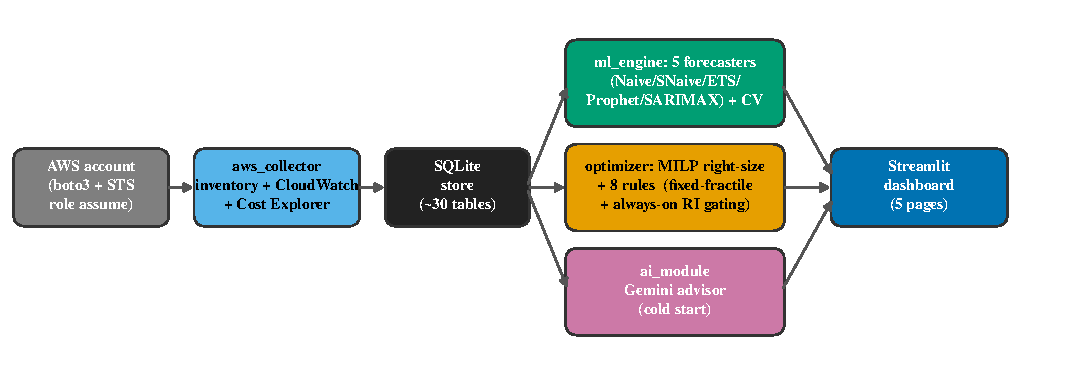
\includegraphics[width=\columnwidth]{fig_architecture.pdf}
\caption{Smart Cloud Optimizer architecture. The system loads telemetry into
SQLite and runs forecasting, MILP right-sizing, transparent rules, and an LLM
advisor; only right-sizing and reservation behavior are evaluated here.}
\label{fig:arch}
\end{figure}

\subsection{Forecasting and Anomaly Context}
The forecasting module exposes a shared fit/predict interface for Naive,
SeasonalNaive, ETS, Prophet, and SARIMAX models. Paper scripts evaluate them
with walk-forward MAPE, MASE~\cite{hyndman2006mase}, interval coverage, and
small-sample Diebold-Mariano tests~\cite{diebold1995comparing,harvey1997testing}.
Forecasts support monitoring context; sizing uses observed utilization
percentiles, which matters because real-trace aggregate forecasts are weak.

\subsection{MILP Right-Sizing}
For compute resources, the optimizer solves a binary assignment problem. Let
$\mathcal{I}$ be resources and $\mathcal{C}$ candidate instance types with
price $p_c$, vCPUs $v_c$, and memory $m_c$. The decision variable
$x_{i,c}\in\{0,1\}$ assigns resource $i$ to type $c$:
\begin{align}
\min_x \quad & \sum_{i\in\mathcal{I}}\sum_{c\in\mathcal{C}} p_c x_{i,c}\\
\mathrm{s.t.}\quad & \sum_c x_{i,c}=1 && \forall i,\\
& \sum_c v_c x_{i,c}\ge r_i^{cpu} && \forall i,\\
& \sum_c m_c x_{i,c}\ge r_i^{mem} && \forall i,\\
& \sum_{i,c} p_c x_{i,c}\le B && \mathrm{if\ a\ cap\ is\ supplied}.
\end{align}
The requirement $r_i$ uses the deployed rule:
\begin{equation}
r_i = q_{0.95}(u_i)\,V_i\,h,\qquad h=1.3,
\end{equation}
where $u_i$ is observed utilization and $V_i$ is current capacity. EC2 uses
CPU and memory when memory utilization is available; RDS uses CPU because the
stored RDS memory metric is not directly comparable as a utilization
percentage.

\subsection{Rule-Based Recommendations}
The rule engine adds transparent service-specific actions such as EC2/RDS
reserved-pricing switches and waste-removal checks, deduplicating by resource
and action type. These rules provide implementation context; the paper's
quantitative claims come from the MILP, generated evidence tables, and
reservation-policy simulations.

\section{Reservation-Fractile Interpretation}

The system's high-percentile rule is conservative by design. It aims to avoid
performance-impacting under-provisioning when choosing instance sizes. For
reservation sizing, however, the cost model is different. If a reserved unit
costs $w_T$ per period and on-demand costs $w_0$, define
$\gamma=w_T/w_0$. A static reserved capacity $K$ charged against demand $D$
has normalized expected cost
\begin{equation}
C(K)=\gamma K+\E\pos{D-K}.
\end{equation}
The newsvendor optimum chooses the empirical $(1-\gamma)$ quantile. Thus, at
$\gamma\approx\polGammaStar$, the optimal reservation service level is far
below $0.95$. This does not invalidate P95 right-sizing. It means that a P95
capacity guardrail and a reservation commitment level solve different
problems.

The policy simulation in Section~\ref{sec:policy} makes this distinction
quantitative. It reads the deployed $q_{0.95}\times1.3$ rule counterfactually
as if it were a reservation-sizing rule, then compares it with the newsvendor
fractile, a sample-average-approximation stochastic program, dual-capacity
base/surge policies, look-back replay policies, and a clairvoyant lower bound.

\section{Experimental Design}

\subsection{Research Questions}
The evaluation is organized around four questions:
\begin{itemize}
\item RQ1: What savings does the implemented optimizer report on the
repository's synthetic AWS account?
\item RQ2: Does the same MILP right-sizing rule transfer to public real VM
traces under a consistent price catalog?
\item RQ3: How reliable are the forecasting models as a basis for capacity
planning?
\item RQ4: What is the out-of-sample cost of applying a conservative
right-sizing fractile to reservation sizing?
\end{itemize}

\subsection{Datasets and Inputs}
Table~\ref{tab:datasets} summarizes the datasets used by the paper scripts.
Study I uses the committed synthetic AWS account. Study II uses public
Bitbrains and Materna traces~\cite{shen2015bitbrains,iosup2008gwa}, priced
against a verified AWS catalog snapshot. The Azure arm uses the Azure Public
Dataset V2 lineage associated with Resource Central~\cite{cortez2017resource}.

The study uses the GWA fastStorage, GWA Rnd, and GWA Materna traces; the
retained Azure aggregate artifact; synthetic account data; the documented AWS
price/catalog snapshot; and the derived evidence files recorded in the
repository. For the synthetic-account arm, publicly available workload traces
and catalog artifacts were processed and organized into a unified synthetic
account-level environment with generated resource identifiers. The workloads
were assigned across a deliberately complex EC2/RDS-style infrastructure to
support controlled evaluation of the implemented optimization workflow. The
environment simulates selected structural characteristics of an AWS account
but is not a live production account and contains no customer or personal
data. The resulting account-level data are synthetic; they are not output from
AWS, Azure, or another commercial recommender.

\begin{table*}[t]
\caption{Evaluation inputs. GWA checksums and provenance are recorded in
\texttt{trace\_provenance.md}; the Azure raw-input checksum remains unavailable.}
\label{tab:datasets}
\centering
\renewcommand{\arraystretch}{1.12}
\resizebox{\textwidth}{!}{%
\begin{tabular}{@{}l l l l@{}}
\toprule
Input & Scale and period & Used for & Evidence file \\
\midrule
Synthetic AWS account & \nDays{} days (\dataStart--\dataEnd), \numResources{} resources & optimizer savings, forecasting, policy simulation & \texttt{results\_baselines.json}; \texttt{results\_ablations.json}; \texttt{numbers\_evidence.tex}; \texttt{table\_service\_decomposition.tex}; \texttt{results\_catalog\_comparison.json} \\
Bitbrains fastStorage & \extFsVms{} VMs, 2013 trace & real-trace MILP right-sizing & \texttt{results\_external.json}; \texttt{trace\_provenance.md} \\
Bitbrains Rnd & \extRndVms{} VMs, \extRndHours{} hourly aggregate points & right-sizing, forecasting, policy simulation & \texttt{trace\_rnd\_hourly.csv}; \texttt{trace\_provenance.md} \\
Materna-Trace-3 & \extMatVms{} VMs, 2016 trace & second-provider right-sizing validation & \texttt{results\_external.json}; \texttt{trace\_provenance.md} \\
Azure Public Dataset V2 & \azVms{} filtered VMs from \azTotalRows{} rows, 2019 trace & boundary-condition right-sizing study & \texttt{results\_azure.json}; raw input not restored \\
\bottomrule
\end{tabular}}
\end{table*}

\subsection{Metrics}
Optimization results are reported as estimated monthly cost reduction relative
to the relevant baseline. Forecasting uses MAPE, MASE, empirical interval
coverage, and paired statistical tests where enough aligned forecast errors
exist. Policy-simulation results are normalized as realized test cost as a
percentage of an on-demand-only baseline.

\subsection{Generated Baselines and Ablations}
Tables~\ref{tab:baselines}--\ref{tab:runtime} are generated by
\texttt{paper/evidence\_experiments.py}. The baseline and ablation rows use
the committed synthetic account, but EC2 current inventory and EC2 candidates
are repriced to the same snapshot AWS catalog so current and recommended costs
are comparable. RDS remains on the committed demo DB price basis because the
paper snapshot covers EC2 only. EC2 right-sizing costs are evaluated on a
common snapshot on-demand price basis so that capacity choices are
comparable, including two \texttt{m5.xlarge} current-inventory rows originally
recorded at RI prices; reserved-instance commitment effects are evaluated
separately in the paper-side usage-hour RI replay surrogate and in Study III. This
normalization does not mean the originally reserved EC2 inventory would
actually be billed at on-demand rates, and it is not a claim about AWS Cost
Explorer, Savings Plans, or commercial recommender output. If a service-level
MILP is infeasible, the table marks the row as partial or failed and does not
report a comparable savings percentage. The restored GWA raw-trace rerun adds
Study II bootstrap intervals and a percentile baseline grid in
\texttt{results\_external.json} and
\texttt{table\_external\_baselines.tex}; the Azure raw
\texttt{vmtable.csv.gz} remains absent. Table~\ref{tab:commercial-like}
reports a
labeled usage-hour reservation replay surrogate; it is not a commercial-tool
output.

\subsection{Candidate Catalog Completeness}
The synthetic-account ablations expose a feasibility boundary in the committed
demo catalog. The evidence script records 13 EC2 price rows in the database,
but only four EC2 rows have the positive price and hardware specifications
needed by the implemented MILP; RDS has six price rows and four solver-valid
rows. Under $q_{0.95}\times1.3$ and related high-percentile or high-headroom
settings, the EC2 constraints exceed that reduced candidate set, so CBC
returns an infeasible EC2 assignment while the RDS subproblem remains feasible.
This is a catalog-completeness and constraint-feasibility boundary, not a
claim that conservative P95 sizing is universally infeasible.

To separate catalog coverage from policy infeasibility,
\texttt{paper/catalog\_comparison.py} reruns the same baseline and ablation
grid while repricing EC2 current inventory and EC2 candidates with the
documented, snapshot-dated 28-type AWS Price List catalog used by the
external-validation scripts. RDS candidates remain unchanged.
Table~\ref{tab:catalog-comparison} shows that
the non-budget EC2 infeasibilities disappear under this richer EC2 candidate
set. The remaining EC2 infeasibilities are confined to explicit budget-cap
rows, where the conservative snapshot-priced EC2 assignment exceeds the EC2
service-level cap. The paper can safely
conclude that production right-sizing pipelines must validate catalog coverage
and budget feasibility before applying aggressive headroom policies. It still
cannot conclude that a full all-SKU AWS catalog, AWS Compute Optimizer, Azure
Advisor, or a commercial FinOps tool would behave the same way.

\begin{table*}[t]
\caption{Catalog-comparison rerun for the synthetic-account EC2 feasibility boundary. The snapshot row uses a shared EC2 price basis: current EC2 inventory and EC2 candidates are repriced with the documented AWS Price List snapshot in \texttt{aws\_catalog.py}; RDS candidates remain from the committed demo database. The 19.0\% snapshot-row saving is the service-mixed aggregate decomposed in Table~\ref{tab:service-decomp}. Non-cap EC2 infeasible rows exclude explicit budget-cap constraints. Partial rows are not comparable savings estimates.}
\label{tab:catalog-comparison}
\centering
\renewcommand{\arraystretch}{1.08}
\resizebox{\textwidth}{!}{%
\begin{tabular}{@{}l r r l r r r r l@{}}
\toprule
Catalog/basis & EC2 raw & EC2 valid & P95$\times$1.3 status & Cost & Saving & Non-cap EC2 infeas. & Cap EC2 infeas. & Boundary \\
 & & & & (\$/mo) & (\%) & rows & rows & \\
\midrule
Original demo DB & 13 & 4 & Partial (EC2 Infeasible) & -- & -- & 9/18 & 4/4 & catalog coverage \\
AWS snapshot shared EC2 basis & 28 & 28 & Optimal & 1,006 & 19.0 & 0/18 & 4/4 & service budget cap \\
\bottomrule
\end{tabular}}
\vspace{0.25em}
\begin{minipage}{0.98\textwidth}
\footnotesize
EC2 infeasibility disappears for non-budget baseline and ablation rows with the shared-basis snapshot EC2 catalog; remaining EC2 infeasibility is confined to explicit per-service budget-cap rows.
\end{minipage}
\end{table*}


\begin{table*}[t]
\caption{Generated baseline comparison. Synthetic compute rows use a shared price basis: EC2 current inventory and EC2 candidates are repriced with the snapshot-dated AWS catalog in \texttt{paper/aws\_catalog.py}; RDS remains on the committed demo DB basis because the paper snapshot covers EC2 only. Aggregate synthetic savings, including the 19.0\% P95 x 1.3 row, should be read with the EC2/RDS split in Table~\ref{tab:service-decomp}. Partial or failed rows are not comparable savings estimates and are shown as ``--''. The real-trace row uses the restored GWA Study II lift-and-shift aggregate; the full GWA baseline grid is in \texttt{table\_external\_baselines.tex}. Bootstrap intervals are descriptive resource-level 95\% intervals.}
\label{tab:baselines}
\centering
\renewcommand{\arraystretch}{1.08}
\begin{tabular}{@{}l r r r r r r l@{}}
\toprule
Method & Resources & Cost & Saving & 95\% CI & Down & Up & Status \\
 & & (\$/mo) & (\%) & (\%) & & & \\
\midrule
Current inventory & 10 & 1,242 & 0.0 & [0.0, 0.0] & 0 & 0 & Baseline \\
Mean utilization & 10 & 347 & 72.0 & [48.0, 85.5] & 9 & 0 & Optimal \\
Median utilization & 10 & 332 & 73.3 & [50.5, 86.4] & 9 & 0 & Optimal \\
P90 sizing & 10 & 660 & 46.8 & [17.5, 74.9] & 9 & 0 & Optimal \\
P95 sizing & 10 & 660 & 46.8 & [17.5, 74.9] & 9 & 0 & Optimal \\
P95 x 1.3 heuristic & 10 & 1,006 & 19.0 & [-48.0, 72.5] & 8 & 2 & Optimal \\
P99 sizing & 10 & 660 & 46.8 & [17.5, 74.9] & 9 & 0 & Optimal \\
Max utilization & 10 & 736 & 40.7 & [10.3, 69.2] & 7 & 0 & Optimal \\
\midrule
Lift-and-shift to P95 x 1.3 & 2297 & 126,426 & 41.8 & -- & 1575 & 242 & existing aggregate; raw per-VM CI not rerun \\
\bottomrule
\end{tabular}
\end{table*}


\begin{table}[t]
\caption{Study I service-level decomposition for the generated $q_{0.95}\times1.3$ row. EC2 current inventory and candidates use the shared snapshot on-demand basis; RDS remains on the committed demo DB basis. Positive deltas indicate cost increases.}
\label{tab:service-decomp}
\centering
\renewcommand{\arraystretch}{1.06}
\begin{tabular}{@{}l r r r r@{}}
\toprule
Scope & Current & Optimized & Delta & Delta \\
 & (\$/mo) & (\$/mo) & (\$/mo) & (\%) \\
\midrule
EC2 & 844 & 971 & +127 & +15.0 \\
RDS & 398 & 35 & -363 & -91.2 \\
Aggregate & 1,242 & 1,006 & -236 & -19.0 \\
\bottomrule
\end{tabular}
\end{table}


\begin{table*}[t]
\caption{Generated ablation results on the synthetic account with EC2 repriced to the snapshot AWS catalog. Percentile, headroom, memory, and budget rows report assignment cost only for feasible MILP solves; aggregate 19.0\% rows inherit the EC2/RDS split and RDS demo-price caveat in Table~\ref{tab:service-decomp}. Partial or failed rows expose feasibility limits and are not comparable savings estimates. Rule-set rows are a recomputed implementation sanity check on the committed demo DB, not the source of headline paper savings.}
\label{tab:ablations}
\centering
\renewcommand{\arraystretch}{1.06}
\resizebox{\textwidth}{!}{%
\begin{tabular}{@{}l l r r r r l@{}}
\toprule
Dimension & Level & Cost & Saving & CPU exceed & Recs/vars & Status \\
 & & (\$/mo) & (\%) & (\%) & & \\
\midrule
percentile q & 0.75 & 478 & 61.5 & 1.2 & 232 & Optimal \\
percentile q & 0.90 & 1,006 & 19.0 & 0.0 & 232 & Optimal \\
percentile q & 0.95 & 1,006 & 19.0 & 0.0 & 232 & Optimal \\
percentile q & 0.99 & 1,141 & 8.1 & 0.0 & 232 & Optimal \\
headroom h & 1.0 & 660 & 46.8 & 0.0 & 232 & Optimal \\
headroom h & 1.1 & 660 & 46.8 & 0.0 & 232 & Optimal \\
headroom h & 1.3 & 1,006 & 19.0 & 0.0 & 232 & Optimal \\
headroom h & 1.5 & 1,141 & 8.1 & 0.0 & 232 & Optimal \\
memory constraint & off & 585 & 52.9 & 0.0 & 232 & Optimal \\
memory constraint & observed & 1,006 & 19.0 & 0.0 & 232 & Optimal \\
budget cap & none & 1,006 & 19.0 & 0.0 & 232 & Optimal \\
budget cap & 100\% current & -- & -- & -- & 232 & Partial (EC2 Infeasible) \\
budget cap & 90\% current & -- & -- & -- & 232 & Partial (EC2 Infeasible) \\
budget cap & 75\% current & -- & -- & -- & 232 & Partial (EC2 Infeasible) \\
budget cap & 1\% current & -- & -- & -- & 232 & Failed (EC2 Infeasible, RDS Infeasible) \\
\midrule
rule set & MILP right-sizing only & -- & -- & -- & 2 & \$362.81/mo \\
rule set & reserved pricing only & -- & -- & -- & 2 & \$125.85/mo \\
rule set & waste rules only & -- & -- & -- & 11 & \$19.17/mo \\
rule set & all rules, deduplicated & -- & -- & -- & 15 & \$507.83/mo \\
\bottomrule
\end{tabular}}
\end{table*}


\begin{table}[t]
\caption{Runtime and clone-stress diagnostics for the generated evidence script. GWA Bitbrains/Materna raw-trace parsing runtimes are recorded in \texttt{trace\_provenance.md}; Azure raw parsing runtime was not recorded because the raw \texttt{vmtable.csv.gz} input was not restored. These diagnostics are not a hardware-normalized scalability study.}
\label{tab:runtime}
\centering
\renewcommand{\arraystretch}{1.06}
\resizebox{\columnwidth}{!}{%
\begin{tabular}{@{}l r r r r r l@{}}
\toprule
Experiment & $n$ & Vars & Solves & Solve s & Peak MB & Status \\
\midrule
baseline sweep & 10 & 1624 & 14 & 0.117 & 114.1 & computed \\
ablation sweep & 10 & 3480 & 30 & 0.248 & 118.6 & computed \\
rule-set ablation & 10 & 0 & 0 & 0.557 & 118.6 & computed \\
EC2 MILP stress n=100 & 100 & 2800 & 1 & 0.071 & 120.4 & Optimal \\
EC2 MILP stress n=500 & 500 & 14000 & 1 & 0.396 & 141.5 & Optimal \\
EC2 MILP stress n=1000 & 1000 & 28000 & 1 & 1.285 & 171.4 & Optimal \\
evidence script total & 10 & 49904 & 47 & 7.860 & 171.4 & computed \\
\bottomrule
\end{tabular}}
\end{table}


\begin{table}[t]
\caption{Paper-side EC2 usage-hour RI replay baseline. The replay uses trailing observed metric coverage and the same snapshot EC2 on-demand/reserved prices; it is not AWS Compute Optimizer, Cost Explorer, Azure Advisor, or third-party recommender output. The 7-, 30-, and 60-day windows collapse to one row because they select the same six fully observed synthetic EC2 instances.}
% Deprecated commercial-like packaging label retained for the finalized conference source.
\label{tab:commercial-like}
\centering
\renewcommand{\arraystretch}{1.06}
\begin{tabular}{@{}l r r r r l@{}}
\toprule
Lookbacks & Recs & Current & Saving & Saving & Status \\
(days) & & (\$/mo) & (\$/mo) & (\%) & \\
\midrule
7/30/60 & 6 & 563 & 209 & 37.1 & paper-side replay \\
\bottomrule
\end{tabular}
\end{table}


\section{Results}

\subsection{Study I: Synthetic AWS Account}
The synthetic account spans \nDays{} days from \dataStart{} to \dataEnd{}.
The pricing audit in \texttt{paper/pricing\_audit.md} shows that the stored
EC2 current-inventory costs are mostly consistent with the snapshot catalog,
but several committed \texttt{instance\_pricing} candidate rows are wrong or
incomplete. Consequently, the paper does not use the stale stored
\texttt{recommendations} table as a headline savings result. The recomputed
implementation sanity check emits \evidRuleRecs{} deduplicated recommendations
worth \$\evidRuleSavings{}/mo under the committed demo DB path; this is kept
as system-context evidence, not as the paper's primary price-comparable
right-sizing result.

On the corrected compute-scope price basis, current synthetic compute cost is
\$\evidComputeCurrent{}/mo. The deployed $q_{0.95}\times1.3$ MILP row is
feasible and costs \$\evidPfiveCost{}/mo. Table~\ref{tab:service-decomp}
shows why the aggregate \evidPfiveSavingsPct\% reduction is not an
unqualified optimizer win: EC2 increases from \$\evidEcTwoCurrent{}/mo to
\$\evidEcTwoOptimized{}/mo, a \$\evidEcTwoDelta{}/mo
(\evidEcTwoDeltaPct\%) increase, while RDS decreases from
\$\evidRdsCurrent{}/mo to \$\evidRdsOptimized{}/mo, a
\$\evidRdsSavings{}/mo (\evidRdsSavingsPct\%) decrease. Since RDS remains on
the committed demo DB price basis, the aggregate reduction should be read as
a method-illustrative service-mix result. The EC2 increase is the more direct
evidence for the paper's boundary condition: conservative headroom can upsize
capacity and reduce or reverse service-level savings.

The usage-hour replay surrogate recommends \evidCommercialRecs{} EC2
reservations over the \evidCommercialLookbacks{} day look-back windows,
saving \$\evidCommercialSavings{}/mo (\evidCommercialSavingsPct\%) on
eligible EC2 on-demand spend. The rows collapse because all six eligible
synthetic on-demand EC2 instances have full metric coverage in every window
and the snapshot reserved/on-demand prices are static. These are synthetic,
method-illustrative estimates and not realized production savings.

Forecasting is useful but not decisive for the cost results. Table~\ref{tab:mape}
shows walk-forward MAPE on the synthetic account. ETS has the best mean at
the 30-day horizon (\mapeEts\%), but the ETS versus seasonal-naive difference
is not statistically significant at the reported sample size
($p=\dmPEtsSnaive$). The paper therefore treats ETS as the selected model for
monitoring, not as proof of forecasting superiority.

Tables~\ref{tab:baselines} and~\ref{tab:ablations} further qualify Study I.
The generated baseline table uses the snapshot EC2 current/candidate basis,
where the non-budget $q_{0.95}\times1.3$ row is feasible. The catalog
comparison in Table~\ref{tab:catalog-comparison} preserves the original demo
catalog outcome: with only four solver-valid EC2 candidates, the EC2
subproblem is infeasible under the same policy while RDS remains feasible.
Partial original-demo rows are therefore marked as non-comparable savings
estimates; fallback costs are retained only in JSON diagnostics. These rows
should be read as a feasibility boundary condition, not as evidence of a
complete EC2 right-sizing solution or as a universal failure of P95
right-sizing. Replacing the incomplete demo EC2 catalog with the documented
28-type snapshot EC2 candidate set makes the non-budget P95 and
high-percentile/headroom rows feasible, while explicit per-service budget caps
remain a separate infeasibility boundary.

\begin{table}[t]
\caption{Study I synthetic-account walk-forward MAPE (\%, mean $\pm$ sd).
The source table is generated by \texttt{make\_figures.py}.}
\label{tab:mape}
\centering
\renewcommand{\arraystretch}{1.10}
\setlength{\tabcolsep}{3pt}%
\resizebox{\columnwidth}{!}{%
\begin{tabular}{@{}l r r r r r @{}}
\toprule
Model & $h{=}7$ & $h{=}14$ & $h{=}30$ & $h{=}60$ & $h{=}90$ \\
\midrule
ETS (selected)   & 11.28 $\pm$ 2.54 & 11.24 $\pm$ 2.45 & \textbf{11.20 $\pm$ 0.57} & \textbf{11.39 $\pm$ 0.74} & \textbf{12.15 $\pm$ 2.39} \\
SeasonalNaive    & \textbf{10.18 $\pm$ 2.84} & \textbf{10.84 $\pm$ 2.75} & 12.28 $\pm$ 2.82 & 12.66 $\pm$ 2.21 & 12.91 $\pm$ 2.02 \\
Prophet          & 14.41 $\pm$ 6.22 & 20.47 $\pm$ 7.40 & 20.93 $\pm$ 7.53 & 19.70 $\pm$ 7.89 & 18.08 $\pm$ 8.42 \\
Naive            & 25.16 $\pm$ 4.47 & 27.90 $\pm$ 3.52 & 27.26 $\pm$ 4.36 & 27.87 $\pm$ 4.09 & 27.38 $\pm$ 3.70 \\
\bottomrule
\end{tabular}}

\end{table}

\subsection{Study II: External Real-Trace Validation}
Table~\ref{tab:external} reports real-trace right-sizing from restored GWA
raw traces. The baseline maps each VM to the cheapest AWS type covering
provisioned cores and memory. The optimized assignment uses the deployed
$q_{0.95}\times1.3$ requirements. On Bitbrains fastStorage and Rnd,
right-sizing saves \extFsSavingsPct\% (95\% CI
\extFsSavingsCiLow--\extFsSavingsCiHigh\%) and \extRndSavingsPct\%
(\extRndSavingsCiLow--\extRndSavingsCiHigh\%), respectively. On Materna, the
saving is \extMatSavingsPct\% (\extMatSavingsCiLow--\extMatSavingsCiHigh\%),
reflecting much larger over-provisioning in that trace. Across all restored
GWA VMs, the aggregate saving is \extOverallSavingsPct\%
(\extOverallSavingsCiLow--\extOverallSavingsCiHigh\%). Applying one-year
reserved pricing to the optimized always-on trace fleet raises total
reductions to \extFsSavingsPctRi\%, \extRndSavingsPctRi\%, and
\extMatSavingsPctRi\%. Using one-year RI pricing, the pooled mapped reduction
is \extOverallSavingsPctRi\% (95\% CI
\extOverallSavingsPctRiCiLow--\extOverallSavingsPctRiCiHigh\%).

\begin{table}[t]
\caption{Study II restored-GWA right-sizing at AWS on-demand rates from
snapshot \extSnapshot. The $+$RI column applies one-year reserved pricing.}
\label{tab:external}
\centering
\renewcommand{\arraystretch}{1.08}
\setlength{\tabcolsep}{3.5pt}
\begin{tabular}{@{}l r r r r@{}}
\toprule
Dataset & VMs & Baseline & Optimized & Saving / $+$RI \\
 & & (\$/mo) & (\$/mo) & (\%) \\
\midrule
fastStorage & \extFsVms{} & \extFsBaseline{} & \extFsOptimized{} & \extFsSavingsPct{} / \extFsSavingsPctRi{} \\
Rnd & \extRndVms{} & \extRndBaseline{} & \extRndOptimized{} & \extRndSavingsPct{} / \extRndSavingsPctRi{} \\
Materna & \extMatVms{} & \extMatBaseline{} & \extMatOptimized{} & \extMatSavingsPct{} / \extMatSavingsPctRi{} \\
\bottomrule
\end{tabular}
\end{table}

\begin{table}[t]
\caption{Study II GWA baseline grid: savings vs. lift-and-shift (\%). Full CIs
and costs are in \texttt{table\_external\_baselines.tex}.}
\label{tab:external-baselines}
\centering
\scriptsize
\renewcommand{\arraystretch}{1.03}
\setlength{\tabcolsep}{2.6pt}
\begin{tabular}{@{}l r r r@{}}
\toprule
Policy & fastStorage & Rnd & Materna \\
\midrule
Lift-and-shift & 0.0 & 0.0 & 0.0 \\
Mean & 81.4 & 82.6 & 86.1 \\
Median & 86.8 & 90.4 & 86.5 \\
P90 & 46.6 & 42.0 & 81.4 \\
P95 & 40.2 & 37.4 & 78.8 \\
P99 & 34.0 & 32.1 & 73.3 \\
Max & 7.3 & -3.7 & 42.7 \\
P95 x 1.3 & 33.6 & 33.1 & 74.2 \\
\bottomrule
\end{tabular}
\end{table}


Table~\ref{tab:external-baselines} shows that mean, median, and
less-conservative percentile sizing can produce higher apparent mapped savings than
$q_{0.95}\times1.3$. This does not make them better policies by itself: the
paper does not yet evaluate SLO or performance-risk violations after
right-sizing. The result instead exposes the savings-risk frontier central to
the paper: conservative headroom reduces risk exposure but can sacrifice
savings, so P95 x 1.3 should not be oversold as savings-optimal.

The Azure study is deliberately included as a negative boundary condition, but
it was not rerun in this workspace because the raw V2
\texttt{vmtable.csv.gz} input is absent. The committed generated result retains
\azVms{} filtered VMs. Since Azure publishes a max-based CPU percentile and no
per-VM memory-usage series in the vmtable input, memory is held at the
provisioned bucket. Under those semantics, right-sizing alone is cost-negative
(\azSavingsPct\%), although reserved pricing still yields \azSavingsPctRi\%.
This result limits the generality of P95 right-sizing: the rule depends on
what the utilization percentile means and on which resources are measurable.

Forecasting the real aggregate is difficult: at 24 hours the best hourly model
is \extBestModel{} with \extBestMape\% MAPE, and tested pairwise differences
are not statistically significant (e.g., ETS vs. seasonal-naive
$p=\extDmP$). Table~\ref{tab:extmape} supports treating forecasts as
monitoring context rather than savings drivers.

\begin{table}[t]
\caption{Study II real Rnd aggregate forecasting MAPE (\%, mean $\pm$ sd).}
\label{tab:extmape}
\centering
\renewcommand{\arraystretch}{1.08}
\setlength{\tabcolsep}{3pt}
\resizebox{\columnwidth}{!}{%
\begin{tabular}{@{}l r r r r r r @{}}
\toprule
Model & $h{=}6$\,h & $h{=}12$\,h & $h{=}24$\,h & $h{=}48$\,h & $h{=}7$\,d & $h{=}14$\,d \\
\midrule
ETS            & \textbf{48.2 $\pm$ 46.2} & 71.9 $\pm$ 55.4 & 77.0 $\pm$ 57.2 & 91.2 $\pm$ 47.8 & \textbf{52.1 $\pm$ 29.9} & 64.4 $\pm$ 40.9 \\
SeasonalNaive  & 65.9 $\pm$ 33.6 & 73.7 $\pm$ 46.3 & 65.0 $\pm$ 40.3 & \textbf{65.8 $\pm$ 33.8} & 54.2 $\pm$ 22.6 & \textbf{59.7 $\pm$ 32.9} \\
Prophet        & 49.0 $\pm$ 26.2 & \textbf{60.5 $\pm$ 30.0} & \textbf{60.8 $\pm$ 21.6} & 88.1 $\pm$ 42.3 & 59.8 $\pm$ 36.9 & 66.7 $\pm$ 30.0 \\
Naive          & 57.4 $\pm$ 71.2 & 87.9 $\pm$ 86.1 & 82.3 $\pm$ 66.6 & 94.2 $\pm$ 55.7 & 53.4 $\pm$ 14.2 & 66.5 $\pm$ 44.5 \\
\bottomrule
\end{tabular}}

\end{table}

\subsection{Study III: Price of Conservatism}
\label{sec:policy}
The policy simulation splits demand chronologically into train and test
segments, sizes each policy on training data, and charges it on held-out test
demand. The synthetic run uses \polTrainDays{} training days and
\polTestDays{} test days; the real-trace run uses \extPolTrainDays{} training
hours and \extPolTestDays{} test hours. The theoretical formulation expresses
demand and commitment in physical-capacity units. In the empirical
evaluation, the synthetic arm reads daily account cost, so its input series
and commitment proxy are measured in USD/day, whereas the restored Rnd arm is
measured in MHz. The synthetic arm therefore evaluates policy behavior on a
cost-proxy time series rather than simulating physical-capacity allocation or
provider billing. At the catalog reserved/on-demand
ratio $\gamma=\polGammaStar$, the deployed $q_{0.95}\times1.3$ heuristic,
read counterfactually as a reservation-sizing rule, realizes \polPctHeur\%
of on-demand cost on the synthetic account and \extPolPctHeur\% on the real
trace. The newsvendor fractile realizes \polPctNv\% and \extPolPctNv\%.
To avoid comparing only against a deliberately conservative strawman,
Tables~\ref{tab:policy_synth} and~\ref{tab:policy_ext} also include
paper-side 7-, 30-, and 60-day look-back replay policies. These results are
paper-side replay surrogates and are not outputs from AWS, Azure, or another
commercial recommendation system. On the real
trace at $\gamma=\polGammaStar$, the 30-day replay realizes
\extPolPctLookThirty\% of on-demand cost, while the 7-day replay realizes
\extPolPctLookSeven\%, showing that look-back choice matters under bursts.
The real-trace 60-day row equals newsvendor because the training split is
shorter than the requested 60-day window, so the replay uses the full training
set.

Fig.~\ref{fig:policy_synth} and Fig.~\ref{fig:policy_ext} plot the cost curves.
Tables~\ref{tab:policy_synth} and~\ref{tab:policy_ext} give selected
discount levels. The SAA stochastic program recovers the newsvendor quantile
closely, which validates the closed-form policy and the simulator rather
than establishing a separate competing method. The dual-capacity policy adds
little on the synthetic daily series but materially improves the real trace,
where surge states persist long enough for causal activation to retain most
of the value. The look-back rows are therefore a sanity-check replay family,
not a substitute for a direct commercial recommender baseline.

\begin{figure}[t]
\centering
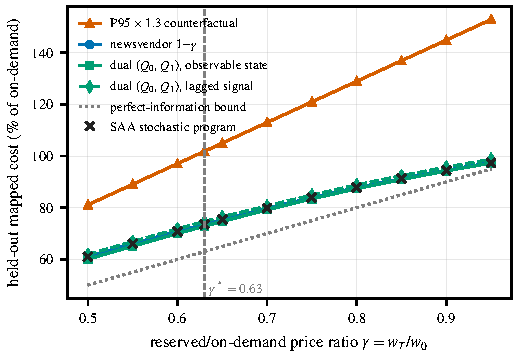
\includegraphics[width=\columnwidth]{fig_policy_gamma.pdf}
\caption{Study III synthetic policy simulation: realized held-out cost as a
percentage of on-demand-only cost across reserved/on-demand ratios.}
\label{fig:policy_synth}
\end{figure}

\begin{figure}[t]
\centering
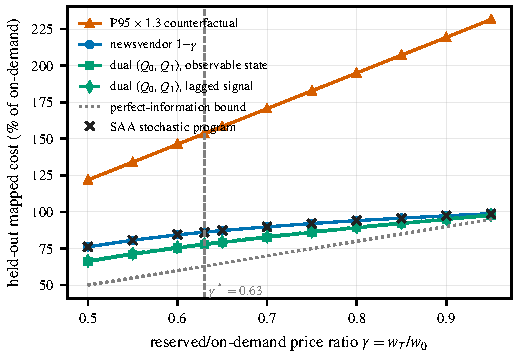
\includegraphics[width=\columnwidth]{fig_policy_gamma_ext.pdf}
\caption{Study III real-trace policy simulation on Bitbrains Rnd aggregate
demand. The dual-capacity variants are most valuable when surge states persist.}
\label{fig:policy_ext}
\end{figure}

\begin{table}[t]
\caption{Study III synthetic policy costs as \% of on-demand-only.}
\label{tab:policy_synth}
\centering
\renewcommand{\arraystretch}{1.08}
\setlength{\tabcolsep}{4pt}
\begin{tabular}{@{}l r r r r @{}}
\toprule
Policy & $\gamma{=}0.60$ & $\gamma{=}0.70$ & $\gamma{=}0.80$ & $\gamma{=}0.90$ \\
\midrule
P95 $\times$ 1.3 counterfactual & 97.0 & 113.0 & 128.9 & 144.9 \\
newsvendor $1{-}\gamma$ & 70.8 & 79.7 & 87.7 & 94.5 \\
SAA stochastic program & 70.8 & 79.8 & 87.8 & 94.5 \\
7-day recency-window replay & 71.0 & 80.2 & 87.6 & 94.5 \\
30-day recency-window replay & \textbf{70.5} & \textbf{79.7} & \textbf{87.4} & \textbf{94.3} \\
60-day recency-window replay & 70.5 & 79.8 & 87.5 & 94.6 \\
dual $(Q_0,Q_1)$, obs.\ state & 70.0 & 79.2 & 87.3 & 94.2 \\
dual $(Q_0,Q_1)$, lagged signal & 71.8 & 80.6 & 88.8 & 95.7 \\
perfect-information bound & 60.0 & 70.0 & 80.0 & 90.0 \\
\bottomrule
\end{tabular}

\end{table}

\begin{table}[t]
\caption{Study III real-trace policy costs as \% of on-demand-only.}
\label{tab:policy_ext}
\centering
\renewcommand{\arraystretch}{1.08}
\setlength{\tabcolsep}{4pt}
\begin{tabular}{@{}l r r r r @{}}
\toprule
Policy & $\gamma{=}0.60$ & $\gamma{=}0.70$ & $\gamma{=}0.80$ & $\gamma{=}0.90$ \\
\midrule
P95 $\times$ 1.3 counterfactual & 146.2 & 170.6 & 195.0 & 219.3 \\
newsvendor $1{-}\gamma$ & 84.4 & 89.8 & 94.1 & 97.4 \\
SAA stochastic program & 84.4 & 89.8 & 94.1 & 97.4 \\
7-day recency-window replay & 89.3 & 95.6 & 102.4 & 103.6 \\
30-day recency-window replay & 82.7 & 89.2 & 93.8 & 97.3 \\
60-day recency-window replay & 84.4 & 89.8 & 94.1 & 97.4 \\
dual $(Q_0,Q_1)$, obs.\ state & 75.4 & 82.7 & 89.2 & 94.9 \\
dual $(Q_0,Q_1)$, lagged signal & \textbf{75.8} & \textbf{83.1} & \textbf{89.6} & \textbf{95.3} \\
perfect-information bound & 60.0 & 70.0 & 80.0 & 90.0 \\
\bottomrule
\end{tabular}

\end{table}

\section{Discussion}

\subsection{What the System Can Safely Claim}
The repository supports three defensible claims. First, the implemented
optimizer combines MILP right-sizing and transparent service rules. Second,
the paper scripts reproduce a multi-part evaluation from database, public
traces, and a snapshot-dated price catalog. Third, the policy simulation
shows that a high right-sizing percentile should not be treated as a
reservation sizing rule without accounting for $\gamma$.

\subsection{What Should Not Be Oversold}
The deployed system does not implement the full dynamic $(s,S)$ policy of
Chen et al.~\cite{chen2024capacity}; it implements static high-percentile
right-sizing and always-on reserved-pricing checks. The LLM advisor is not
evaluated for savings. The external baselines are internal mathematical and
replay baselines, not direct runs of commercial recommenders. Therefore, the
paper should not claim commercial superiority. The synthetic EC2
$q_{0.95}\times1.3$ infeasibility under the committed demo catalog also means
the paper should not present that original EC2 result as a successful
full-fleet EC2 right-sizing solve. The snapshot-catalog rerun supports the
catalog-coverage interpretation, but it is not a commercial-tool or all-SKU
AWS comparison.

\subsection{Artifact Scope and Remaining Extensions}
The minimum synthetic-account baselines, ablations, service decomposition,
and runtime measurements are now generated in
Tables~\ref{tab:baselines}--\ref{tab:runtime}. The catalog comparison in
Table~\ref{tab:catalog-comparison} also reduces the
synthetic EC2 feasibility risk by showing that non-budget infeasibility
disappears under the shared-basis snapshot EC2 candidate set. The
paper-side usage-hour RI replay surrogate in Table~\ref{tab:commercial-like}
partially
addresses the missing-baseline risk but does not replace a direct commercial
tool comparison. The restored GWA Study II rerun adds checksums, bootstrap
intervals, and a baseline grid for Bitbrains and Materna; remaining extensions
include direct commercial baselines, Azure raw-vmtable restoration with timing
and intervals, SLO/performance-risk validation, all-SKU/region catalog
sensitivity, and a full dynamic $(s,S)$ reservation implementation.

\section{Threats to Validity}

\textbf{Synthetic data and demo pricing.} Study I uses the repository's
synthetic AWS account. Its dollar savings are method-illustrative and should
not be presented as production savings. The committed demo EC2 candidate price
table contains incorrect or incomplete rows, so the paper separates original
demo-price diagnostics from snapshot-repriced EC2 results. The aggregate
Study I compute reduction is dominated by RDS, which remains demo-priced; it
should not be used as a production-dollar or cross-service superiority claim.

\textbf{Trace age and mapping.} Bitbrains and Materna are older managed-hosting
traces, and their VMs are priced using a 2026 AWS catalog. The GWA inputs were
restored with checksums for this rerun, but percentages are useful for method
comparison under the mapping, not as absolute production-dollar evidence.

\textbf{Metric semantics.} The Azure result shows that the meaning of a
published percentile matters. Max-based percentiles and unavailable memory
usage can reverse the right-sizing result.

\textbf{Candidate catalog completeness.} The committed synthetic DB contains
more EC2 price rows than solver-valid EC2 hardware rows. Consequently, high
percentile and high-headroom EC2 ablations can be infeasible because the
reduced candidate set cannot satisfy the induced CPU/memory requirements. This
limits synthetic-account conclusions about EC2 right-sizing. The paper-local
catalog comparison reruns the synthetic ablations with a richer 28-type,
snapshot-dated EC2 candidate set and a shared EC2 current/candidate price
basis, and keeps infeasible rows visible. That rerun removes non-budget EC2
infeasibility, but it is still not an all-SKU AWS catalog study and does not
replace a direct commercial recommender baseline.

\textbf{Policy abstraction.} Study III uses aggregate demand and simplified
reservation costs. It does not model all real contract terms, partial upfront
payments, cancellation, resale, instance families, or capacity fragmentation.

\textbf{Baselines.} The SAA baseline is a correctness/replay baseline and
closely matches newsvendor theory by construction. The usage-hour reservation
replay and Study III look-back replay rows are paper-side replay surrogates
only. The paper currently lacks a direct commercial-tool comparison.

\textbf{Statistical power.} Forecasting tests use limited walk-forward folds.
The reported non-significant differences should remain non-claims rather than
being reframed as superiority.

\section{Conclusion}

This paper is best framed as an empirical theory-practice bridge, not as a
product demonstration. Smart Cloud Optimizer operationalizes a FinOps-style
pipeline with forecasting, $q_{0.95}\times1.3$ MILP right-sizing, reserved
pricing checks, and service-specific waste rules. On the repository's
synthetic account, the paper no longer treats the stale stored recommendation
table as a headline savings source; after EC2 snapshot repricing, the
$q_{0.95}\times1.3$ row is feasible but service-mixed: EC2 cost increases by
\evidEcTwoDeltaPct\%, while demo-priced RDS cost decreases by
\evidRdsSavingsPct\%, producing an aggregate compute-scope reduction of
\evidPfiveSavingsPct\%. The aggregate should therefore be interpreted as a
boundary-condition result about conservative headroom and service mix, not as
an unqualified optimizer win. The paper-side reservation replay
surrogate saves \$\evidCommercialSavings{}/mo on eligible EC2 on-demand
spend in a collapsed 7/30/60-day synthetic sanity check. On restored public
Bitbrains and Materna VM traces, the same MILP right-sizing rule saves
\extOverallSavingsPct\% in aggregate against a lift-and-shift baseline
(95\% CI \extOverallSavingsCiLow--\extOverallSavingsCiHigh\%), while the
Azure boundary case, whose raw input was not restored, shows that metric
semantics can make the heuristic fail. The policy simulation then isolates the
central research
insight: under intermittent demand surges, conservative P95-based
right-sizing and price-aware capacity-reservation theory can diverge sharply.
At the observed reserved/on-demand ratio, using the high-percentile capacity
rule as a reservation-sizing rule forfeits the discount, whereas the
newsvendor and look-back replay policies retain much more of it. Remaining
extensions include direct commercial baselines, Azure raw-vmtable restoration
with confidence intervals and runtime measurements, broader all-SKU/region
catalog sensitivity, SLO validation, and live or modern production data.

\section*{Author Contact Information}
\noindent\textbf{Corresponding author:} Ibrahim Mohamed:
\href{mailto:ibrahimmohamedabdelsadek@gmail.com}{\nolinkurl{ibrahimmohamedabdelsadek@gmail.com}}.

\noindent\textbf{Author emails:} Mariam Emad:
\href{mailto:mariamemadcs@gmail.com}{\nolinkurl{mariamemadcs@gmail.com}}; Hazem Ibrahim:
\href{mailto:Ihazem28@gmail.com}{\nolinkurl{Ihazem28@gmail.com}}; Ahmed Sameh:
\href{mailto:ahmed.sameh.12543@gmail.com}{\nolinkurl{ahmed.sameh.12543@gmail.com}}; Mahmoud Ahmed:
\href{mailto:mahmoudkamel9102003@gmail.com}{\nolinkurl{mahmoudkamel9102003@gmail.com}}; John Ehab:
\href{mailto:ehabjohn22@gmail.com}{\nolinkurl{ehabjohn22@gmail.com}}.

\bibliographystyle{IEEEtran}
\bibliography{../references}

\end{document}
